%äöüß
\chapter{Air-Sensitive n-Dopants in \CS}\label{chap:PaddleWheels}
\addcontentsline{lof}{chapter}{\thechapter\hspace*{1ex} Air-Sensitive n-Dopants in \CS}
\addcontentsline{lot}{chapter}{\thechapter\hspace*{1ex} Air-Sensitive n-Dopants in \CS}

%
\intro{This first results chapter studies the properties of n-doped \CS layers incorporating two different n-dopants, \CrPd or \WPd. Both dopants are compounds with extremely low \IEs and thus not stable in air. First, in \secref{ResPdCond} the conductivity of differently doped samples, measured directly after sample preparation is probed. A change over time is observed and modeled theoretically. Afterwards, a thermal annealing step is performed to ensure stable measurement conditions and the influence of the \CLong is analyzed. Finally, temperature-dependent conductivity measurements are discussed, which indicate a thermally activated hopping process and therefore allow to derive an \EactLong. In \secref{ResPd-S}, thermoelectric (Seebeck) measurements are presented and the influence of temperature and \CLong is discussed. The results are compared to the \EactLong and conclusions for the mobility are drawn. \Secref{ResPdAFM} presents atomic force microscopy (AFM) studies, probing the surface roughness of differently doped samples for indications of clustering or agglomeration of dopants. Finally, in \secref{ResPdkilling}
degradation studies of the effect of air-exposure on the n-doped samples are discussed and a regeneration treatment is presented.
This chapter ends with a summary in \secref{ResPdConclusion}.
}

\newpage

% aus Intro
Doping of conventional semiconductors was the key element that led to the breakthrough of semiconductor technology, as it allows for control of the majority charge carriers and hence the design of p-n-junctions, being the building block for most electronic devices. In this chapter, n-doping of the high mobility electron transport material \CS, frequently used in organic photovoltaic cells (OPV), is studied by using two novel n-dopants, \CrPd and \WPd, having extremely low \IEs of \mbox{$\text{IE}=\eV{3.95(13)}$} and \eV{2.68(13)}, respectively. As the IEs of both dopant compounds are determined to be lower than the electron affinity of \CS with \mbox{$\text{EA}=\eV{4.0(3)}$}\cite{Zhao2009}, efficient charge-transfer and therefore effective doping is expected. This fact is especially the case for \WPd, as its IE is even shallower than the IE of the efficient molecular dopant decamethylcobaltocene\footnote{Decamethylcobaltocene is also known as DMC or CoCp$_2^*$, \mbox{$\text{IE}=\eV{3.30}$}\cite{Chan2008}}.
Further details about the materials are
summarized in the materials \secref{Mat}.
A selection of the results presented here is published in reference\cite{Menke2012}.

Samples of \nm{30} thick doped layers are prepared and investigated in vacuum according to sections \ref{sec:ExpSamplePreparation} and \ref{sec:ExpMeasRoutine}. The base pressure during sample procession for the \CrPd samples was \mbox{$\druck\approx\pa{3e-5}$} $(=\SI{3e-7}{\milli\bbar})$. Due to technical problems, for the samples using \WPd, the pressure was one order of magnitude higher, around \mbox{$\druck\approx\pa{3e-4}$}.

\section{Conductivity}\label{sec:ResPdCond}
Conductivity measurements are the first method of choice for studying doping. Therefore, in the following the conductivities \c of layers of \CS n-doped by various \CLongs \C of \CrPd or \WPd are presented. As a linear and symmetric current-voltage relation is measured for all samples, and the reported contact resistance between gold and \CS is low\cite{Kitamura2011}, the charge injection can be neglected. The conductivity data, measured directly after fabrication of the samples at \T[25] is shown in \figref{MR-Cond-n-Pd-evap}.

\cBild[t]
{MR-Cond-n-Pd-evap}
{As-prepared \cLong \vs \CLong}
{As-prepared \cLongL \vs \CLongL of samples of \CS n-doped by \CrPd or \WPd, measured at \T[25]. Compare to undoped \CS with \mbox{$\c\approx \Scm{2e-8}$}\cite{Li2006}.}

Even for the lowest \CLong, the \cLong of the doped layers is several orders of magnitude higher than for undoped \CS, which has been reported to be in the order of \c[2e-8]\cite{Li2006} and which would be below the resolution limit of the setup of \c[8.3e-8] as discussed in \secref{ExpResLimit}.
A linear increase of $\c(\C)$ is observed for both dopants, covering three orders of magnitude. A detailed discussion of the dependence of \c on \C is performed in \secref{ResPdCondMR}, as it is later found that a thermal annealing step is necessary in order to ensure reproducible and stable measurement conditions for later measurements. The maximum conductivity measured directly after sample fabrications is \c[7.35] for \C[0.210] of \CrPd and \c[4.97] for \C[0.150] of \WPd.
At even higher \CLongs the conductivity decreases, which is attributed to high percentages of dopant molecules disturbing the morphology of the host material, hindering the charge carrier transport.

\CS is known for its high electron mobility, compared to other OSCs, which results in such high conductivities. In comparison, the typical OLED electron transport material BPhen\footnote{BPhen is \bphenLong}, for example, reaches conductivities of less than \c[E-6] when doped by Cs$_2$CO$_3$\cite{Park2008}.

\subsection{Conductivity Changes after Preparation}%
\label{sec:ResPdLongTimeCond}
Prior to further measurements, the conductivity of each sample is continuously probed \insitu for 1 hour at a temperature of \T[25]. Interestingly, a change of \c is observed for all samples. While for high \C a drop of \c is detected, a gain is found for low \C. \Figref{MR-LongTimeCond-n-Pd-low-high-fit} compares the normalized changes in \c of a weakly (a) and a strongly (b) doped sample of \CrPd.

\cBild[t]
{MR-LongTimeCond-n-Pd-low-high-fit}
{Conductivity change during first hour after preparation}
{Conductivity changes of samples of \CS doped by \CrPd during the first hour after deposition, continuously measuring \insitu at \T[25]. The \CLongs are (a) \C[0.012] and (b) \C[0.345]. A fit (dashed line) is performed using \eqnref{LongTimeCond-exp}.
}
%
\cBild[t]
{MR-LongTimeCond-n-Pd-fitparameter}
{Conductivity change during first hour after preparation, fitting parameters}
{Fitting parameters of conductivity change during the first hour after sample preparation according to \eqnref{LongTimeCond-exp}: (a) maximal relative change $\chi$ reached after $t\gg\tau$ (b) time constant $\tau$ describing the speed of the change.
}
%

The data can be described by employing a simple model using a differential equation describing population growth for the case of constant generation rate ($c_1$) and population dependent extinction rate ($c_2 \cdot \c(t)$):
\begin{align}
\frac{d\c(t)}{dt} &= c_1 - c_2 \cdot \c(t)
\KOMMA
\\
%
\intertext{which can be solved to}
\frac{\c(t)}{\sigma_0}
&= 1 + \chi \left( 1 - \exp{-\frac{t}{\tau}} \right)
\label{eq:LongTimeCond-exp}
\KOMMA
\end{align}
where $\sigma_0$ is the initial conductivity and $\chi$ is the maximal relative change, reached after a time $t\gg\tau$, with $\tau$ being a time constant describing the speed of the change. The value of $\chi$ is positive for increasing and negative for decreasing conductivity over time. As the dashed fitting lines in \figref{MR-LongTimeCond-n-Pd-low-high-fit} show, the model describes the data well.
Applying this model to the continuous measurements for each sample, the parameters $\chi$ and $\tau$ can be derived, which are summarized in \figref{MR-LongTimeCond-n-Pd-fitparameter}.

% parameter \chi
Both dopants show the same tendency: At low \C, the \insitu conductivity significantly increases during the first hour after sample preparation. Hence, the fitting parameter $\chi$ is positive for these samples, as \figref{MR-LongTimeCond-n-Pd-fitparameter}\,(a) shows. With increasing \C, the magnitude of the change $\chi$ is reduced, reaching negative values for high \Cgr{0.040}. Interestingly, for the samples of the highest conductivities measured directly after sample preparation, a value of $\chi\approx0$ is observed, showing that the conductivity stays almost constant.

% parameter tau
The time constant $\tau$ seems to decrease with rising \C for the \WPd samples, whereas for \CrPd no clear trend is observed. For all samples, $\tau$ varies between 0.25 and 1.5~hours, meaning that for some samples the speed of change is 6~times faster than for others. The sample preparation conditions (rate, homogeneity, pressure, \etc) might have an effect on $\tau$, but so far no simple relation could be found. Thus, an interplay of these parameters might control $\tau$.

In order to verify whether the current flow though the layer is the origin for the change in conductivity, a control measurement is performed on one sample of \C[0.033] of \WPd, %#063,0.0326,4.0)
where instead of continuously measuring, \c is probed only for \sek{20} every 20~minutes. The result is identical, suggesting that the current flow is not the cause of this phenomenon.

\subsection{Relation of Conductivity to Doping Concentration}%
\label{sec:ResPdCondMR}
% \subsection{Thermal Annealing}%
% \label{sec:ResPdAnnealing}
In order to investigate the effect of the change in conductivity in more detail and to ensure stable measurement conditions, the samples are thermally annealed prior to further measurements, as proposed by Nollau\etal\cite{Nollau2000}. They are slowly heated from \T[25] to \grad{100} and kept at this temperature for 20~minutes. Afterwards, the conductivity is found to be constant over time, and the temperature-dependent measurement routine, described in \secref{ExpMeasRoutine}, is started at \T[30].

The conductivity probed at \T[30] after thermal annealing is compared to the initial conductivity measured directly after deposition of the layers (at \T[25]). \Figref{MR-Cond-n-Pd-evapVS30} shows that the same trend is observed for both dopants: While at low \CLongs thermal annealing leads to a gain in \c, at high \C a lowering is found.
Highly doped samples of \CrPd show a much more pronounced effect than samples of \WPd.

The change induced by the thermal annealing is in agreement with the tendency observed during the one hour measurement directly after sample deposition, presented in the last section. This agreement suggests that the annealing accelerates the process responsible for the change of the conductivity after deposition. Only two samples are inconsistent with this trend: The samples of \C[0.045] and \mr{0.097} of \CrPd show a small reduction in \c during the first hour after fabrication at \T[25], but a gain after thermal annealing. This gain is larger than the expected effect of the \K{5} higher temperature for the measurement after annealing.

Three different phenomena might be responsible for the changes in conductivity with time and temperature.
Firstly, residual quantities of gases like O$_2$ and moisture, being present in the vacuum chamber, might react with the n-doped layers, binding electrons and hence reducing the conductivity. Thermal annealing can remove these products from the layer, enhancing the conductivity\cite{Fujimori1994}.
Secondly, in the regime of low \CLong, slow and small rearrangement of the molecules introduced by interactions between host and dopant molecules might lead to an increasing doping efficiency and thus conductivity over time. This effect might be accelerated by thermal annealing.
Thirdly, in the regime of high \CLong, a phase separation and demixing of host and dopant can occur, leading to a reduced conductivity due to shielding of dopants and hence a reduced number of free charges. This rather slow process can be accelerated by heating, as it has been shown for organic photovoltaic cells, where phase separation in the active layer improves the exciton separation by formation of a bulk heterojunction \cite{Suemori2004}.

%
\cBild
{MR-Cond-n-Pd-evapVS30}
{Conductivity before and after thermal annealing}
{Conductivity before (filled symbols, at \T[25]) and after (empty symbols, at \T[30]) thermal annealing (at \T[100]) for \CS doped by (a) \CrPd and (b) \WPd. The dashed lines represent a slope of 1.0.
}
%

After the thermal annealing step, the maximum conductivity measured at \T[30] is \c[4.3] at \C[0.045] of \CrPd, and \c[4.0] at \mr{0.147} of \WPd. As indicated by the dashed lines in \figref{MR-Cond-n-Pd-evapVS30}\,(a) and (b), possessing a slope of 1.0, the conductivity has a linear relation to the \CLong. Hence, each additional dopant molecule contributes by the same amount to the total conductivity. This trend is not always the case, as other studies on organic dopants have shown\cite{Maennig2001,Gregg2004Review}.

A stronger slope might be present in the region of lowest \CLongs for both dopants. This tendency is in agreement with the results Olthof\etal\cite{Olthof2012} have reported for the material system of \CS doped by [RuCp$^*$(mes)]$_2$%
\footnote{[RuCp$^*$(mes)]$_2$ is ruthenium(pentamethylcyclopentadienyl)(1,3,5,-trimethylbenzene)}. A superlinear increase of $\c(\C)$ below \mr{0.001} was observed, which they attributed to filling of trap states. Here, the \CLong is higher, but filling of trap states might also be responsible for the rather low conductivities of the lowest doped samples.

At very large \CLongs \Cgr{0.100}, this linear relation does not hold any more as both sample series show a drop of \c. A possible explanation could be a drop in the electron mobility due to a disturbance of the morphology\cite{Kleemann2012a} when more than 10 dopant molecules per 100 host molecules are introduced into the layer.
As the dopant molecules have different properties than the host molecules, a substitution of molecules leads to a change in the electronic landscape in the layer\cite{Mityashin2012a}.
If deposited dopant molecules preferable align to dopant molecules already present in the layer, at high \C a clustering can happen, leading to a phase separation of host and dopant materials, as discussed above.
For doped layers, a phase separation would result in a reduced doping efficiency as some of the dopant molecules are shielded from the host molecules and thus are not able to donate an electron\cite{Mityashin2012a}. In order to check for possible changes of the layer morphology induced by doping, atomic force microscopy (AFM) measurements are performed using an AIST-NT Combiscope AFM. The measurements are presented in \secref{ResPdAFM} and show a rising roughness with \C in the medium doping regime. Interestingly, at high \C smooth surfaces are found again. This counter-intuitive trend might be a measurement artifact, since the measurements are performed in air.

In contrast to what is expected from the \IEs (IEs), using \CrPd leads to a more efficient doping of \CS compared to \WPd.
Assuming that there is no change of molecular levels on formation of ions, this observation might be explained by morphological effects, or by \WPd reacting more strongly with oxygen contaminations being present in the vacuum chamber.

In order to check if the above mentioned higher pressure during sample procession of \WPd samples had an influence on \c, a sample of \C[0.033] of \WPd is produced at the same pressure as the \CrPd samples, after solving the technical problems. This sample showed after thermal annealing an almost equal conductivity to the earlier \WPd samples of similar \CLong. Again, the conductivity is lower than of a corresponding sample of \CrPd. Hence, the effect of the elevated base pressure seems not to be crucial.

\subsection{Temperature Dependence of the Conductivity}%
\label{sec:ResPdCondEact}
%
Measuring the conductivity (after thermal annealing) at different temperatures, a reversible gain of \c with temperature is observed. \Figref{T-Cond-n-Pd} shows the data of all samples in Arrhenius plots, displaying the conductivity in a logarithmic scale against the reciprocal of the temperature $\T^{-1}$. An exceptionally good agreement with a linear relation is found for all samples, corresponding to an exponential relation of \c to $\T^{-1}$, consistent with earlier studies on doped organic layers\cite{Fujimori1994,Pfeiffer1998}. Thus, this data can be fitted in good agreement with a thermally activated transport relation using \eqnrefPage{CondActivation}. Hence, most likely hopping transport is dominant in these samples and therefore an \EactLong \Eact can be derived.

\cBild[t]
{T-Cond-n-Pd}%
{Temperature dependence of the conductivity}%
{Temperature dependence of the conductivity $\c(T)$ of samples of \CS doped by (a) \CrPd and (b) \WPd. Lines are fits using \eqnrefPage{CondActivation}.}%

\cBild[t]
{MR-Eact-n-Pd}%
{Activation energy of the conductivity}%
{Activation energy of the conductivity \Eact, derived from the temperature dependence of the conductivity $\c(T)$ in the range of \T[30] to \grad{70}, shown above in \figref{T-Cond-n-Pd}, using \eqnrefPage{CondActivation}.
}%

The resulting \Eact of the differently doped samples range from \Eact[54] to \meV{160} and are shown in \figref{MR-Eact-n-Pd}. All obtained values are well below the previously reported value for undoped \CS of around \meV{640}\cite{Li2006}.
At low \C, the \Eact is lower for samples of \CrPd than for \WPd, whereas for \Cgr{0.020}, the values for both dopants match clearly within experimental scattering.
Up to \C[0.100], a decrease of \Eact with increasing \C is found, as expected from earlier experiments\cite{Pfeiffer1998,Li2006}.
Highly doped samples show a different behavior of rising \Eact with \CLong.

The drop of \Eact with increasing \C is attributed to a shift of the \EfLong towards the \EtLong of \CS.
This shift leads to a reduction of the temperature dependence of the \neLong $\ne(T)$, which according to \eqref{Cond-CCD-Mob} contributes to the conductivity as
\begin{equation}
\c(T) = e \cdot \ne(T) \cdot \mobe(T) \tag{\ref{eq:Cond-CCD-Mob}}
\PUNKT
\end{equation}
%
A minimum of \Eact at $\C\approx\mr{0.100}$ suggests a pinning of \Ef and hence a saturation of the doping efficiency.
%
The increase of \Eact at \Cgr{0.100} might be attributed to a rise of the temperature dependence of the electron mobility $\mobe(T)$, probably caused by a disturbance of the morphology of the host material by the large percentage of dopant molecules. Studies on \pen, which forms polycrystalline layers as well, have shown that an increasing amount of dopants leads to a disturbance of the morphology and a decreasing crystallite size\cite{Kleemann2012a}.
The observed rising \Eact is in agreement with the reduced \cLong at \Cgr{0.100}, as shown in \figref{MR-Cond-n-Pd-evapVS30}.

% \newpage

\section{Thermoelectric Measurements}%
\label{sec:ResPd-S}
\subsection{Temperature Dependence of the Seebeck Coefficient}
\label{sec:ResPd-S-T}
\cBild[b]
{T-S-n-Pd}
{Temperature dependence of the Seebeck coefficient}%
{Temperature dependence of the Seebeck coefficient \S for \CS doped by \CrPd and \WPd in (a) and (c). At the right side, in (b) and (d) the relative changes of \S are shown, normalized to the \Tm[40] measurements.
}%
%
Along with the conductivity measurements, thermoelectric (Seebeck) measurements are performed. The measured Seebeck coefficients \S for \CS doped by \CrPd or \WPd are presented in \figref{T-S-n-Pd}\,(a) and (c). They are negative in sign, thus, for all samples, electrons are the dominating charge carrier species and hole conduction along the dopant molecules is not observed. The values for \S range from \uVK{-90} to \uVK{-600} and a lowering of $|\S|$ with rising \C is detected.

In order to investigate the influence of the mean temperature \Tm, the relative changes of \S, normalized to the measurements at \Tm[40], are shown in \figref{T-S-n-Pd}\,(b) and (d) for \CrPd and \WPd, respectively. \Tm[40] is chosen, as it is a device-relevant temperature and more stable to control than \Tm[30]. In the investigated temperature range of \Tm[30] to \grad{70}, the \S of most of the \CrPd samples scatters around relative changes of $-0.5\,\%$ to $+5\,\%$. The two lowest doped samples of \C[0.0020] and \mr{0.0033} are an exception with changes of $-3\,\%$ and $+11\,\%$ at \Tm[70]. In case of using \WPd, most samples show a gain in the order of $4\,\%\pm2\,\%$, with again two weakly doped samples showing stronger changes.

Summarizing, a small upward trend of \S between $2\,\%$ and $6\,\%$ is measured for most samples with no direct relation to the \CLong. It is not clear why weakly doped samples differ from the general trend.
Since the influence of the \CLong on \S is much more pronounced than the effect of the temperature, a comparison of differently doped samples is performed in the next section.

\subsection{Relation of Seebeck Coefficient to Doping Concentration}%
\label{sec:ResPd-S-MR}
\cBild[b]
{MR-See+Es-n-Pd}%
{Seebeck coefficient and derived \EsLong}
{Seebeck coefficient \S and derived \EsLongL at \Tm[40].
}
%
In \figref{MR-See+Es-n-Pd}, the Seebeck coefficients \S at \Tm[40] are compared for different \CLongs. A decrease of $|\S|$ with increasing \C is found for both dopants, ranging from \uVK{-585} to \uVK{-93}.
By using \eqnrefPage{S-Es-org}, the energetic difference \Es between the \EfLong \Ef and the \EtLong \Et is derived:
\begin{align}
 \Es =\S \cdot e \cdot \T \quad \text{ with } \quad\Es := \Ef - \Et
\tag{\ref{eq:S-Es-org}}
\PUNKT
\end{align}
This quantity is shown as the right hand axis in \figref{MR-See+Es-n-Pd}. A maximum of \Es[-183] is measured for \C[0.002] of \CrPd. For \WPd, the largest \Es of \meV{-167} is measured for the lowest concentration (\C[0.004]) as well.

Following the trend of \S, the value of \Es drops with rising \C for both dopants, showing a shift of the \EfLong \Ef towards the \EtLong \Et. A similar tendency has been reported earlier for other material systems\cite{Nollau2000}.
%
A value of \mbox{$\Es<\meV{50}$} is found at high \C for both dopants, which indicates that \Ef is energetically close to \Et at a difference below \mbox{$2\,\kT$}. In such a case, \Ef can get pinned close to \Et which will result in a saturation of \Es, compare degenerate doping in \secref{TheoDegenerateDoping}.
While for \CSCs the Seebeck coefficient at very high \CLongs has been reported to increase again\cite{Ikeda2010}, this behavior is not observed in this data.

Using the Boltzmann approximation, the \neLong $\ne(T)$ is found to be related to \Es via \eqnrefPage{n-von-Es-org-prop}:
\begin{equation*}
\ne(T) \propto \exp{-\frac{|\Es(T)|}{\kT}}
% \tag{\ref{eq:n-von-Es-org-prop}}
\PUNKT
\end{equation*}
Hence, a decreasing value of \Es is attributed to an increasing \neLong.
In case of highly doped samples, $|\Es|$ is in the order of \mbox{$2\,\kT$} and therefore the Boltzmann approximation is not valid, but still a lowering of $|\Es|$ is correlated to a drop of \ne, as discussed in \secref{TheoTempDepMob}.

It can be summarized that the Seebeck coefficient tends towards saturation at high \CLongs of each dopant, \CrPd and \WPd. This saturation is explained by pinning of the \EfLong close to the \EtLong at these high \CLongs.

% \pagebreak
% \subsection[Comparison of \texorpdfstring{\Es}{Es} and \texorpdfstring{\Eact}{Eact}]
% {Comparison of \boldmath \Es and \Eact}
\subsection{Comparison of Seebeck Energy and Activation Energy}
\label{sec:ResPd-EsEact}
%
In \figref{MR-Es+Eact-Pd}\,(a) and (b), the \EsLongL (energetic difference between \EfLongL and \EtLongL) and the \EactLongL, are illustrated for samples doped by \CrPd and \WPd, respectively. A good agreement of the two energies is observed for \Ckl{0.100} of each dopant. At higher \CLongs, an increasing difference is measured, due to a rise in \Eact, as discussed in \secref{ResPdCondEact}. % This finding is an indication for a contribution of the mobility.
If the mobility $\mob(T)$ has an Arrhenius-like temperature dependence, the difference between \Eact and \Es is attributed to an activation of the mobility, as discussed in \secref{TheoTempDepMob}.

Considering the continuing decrease in the Seebeck coefficient even after \C[0.100], the final gain of \Eact and drop of \cLong at high \CLongs must be due to changes of the value of the mobility in the layer.
At these high \C, a disturbance of the morphology by the large number of dopant molecules is expected, negatively affecting the mobility.
This agrees with the results of Harada\etal\cite{Harada2007} who showed that the OFET-mobility of \aob-doped \CS decreases upon doping. In the following section, AFM studies of the surface roughness are presented to check for the influence of doping on the morphology.

However, the temperature dependence of the mobility may differ from a simple activated case to a model where hopping along a manifold of states is assumed\cite{Bassler1982, Vissenberg1998}. In order to differentiate, it would be necessary to measure the mobility independently, for example by temperature-dependent Hall effect or time of flight (TOF) measurements. Using OFET measurements to derive the mobility of doped layers is delicate, since doping leads to a strong contribution of bulk current to the drain current making the mobility analysis based on the gradual channel approximation ambiguous. Furthermore, the high applied field results in a high occupation of the density of states and hence to different conditions compared to the conductivity and Seebeck measurements.

\cBild[t]
{MR-Es+Eact-Pd}
{Comparison of \Es and \Eact}
{Comparison of \EsLongL and \EactLongL. \Es is measured at \Tm[40], \Eact is fitted from conductivity data in the range of \T[30] to \grad{70}.}

% \pagebreak
\section{Morphology}\label{sec:ResPdAFM}
%
\cBildDraw[p]{afm-Pd-images}%
{AFM images}%
{AFM images of a selection of samples. \mbox{(a-f)}: \CS doped by \CrPd, \mbox{(g-l)}: \CS doped by \WPd. Note the different height scales. Parameters: $\um{2}\times\um{2}$ scan area, \nm{30} layer thickness, measurements performed in air after electrical investigations and thermal annealing.
}%
%
In order to check for an influence of the presence of dopant molecules on the morphology of the layers, atomic force microscopy (AFM) measurements are performed on the surfaces of a selection of the same samples electrically investigated and discussed above. After the electrical measurements, the samples are removed from the vacuum chamber and stored in air for several hours before and during the AFM measurements.
Therefore, the results might differ from freshly prepared samples, measured in an inert atmosphere.

The topographies of selected samples are illustrated in \figref{afm-Pd-images}, each scanned on an area of $\um{2}\times\um{2}$. As a figure of merit, the root-mean-square surface roughness \rms is written onto the images and plotted against the \CLong in \figref{MR-AFM-Pd}.
%
\cBild[t]
{MR-AFM-Pd}%
{AFM root-mean-square surface roughness \rms}
{AFM root-mean-square surface roughness \rms of all measured samples, scanned on an area of $\um{2}\times\um{2}$, as shown in \figref{afm-Pd-images}.
}
%
Most samples show a smooth surface formation with $\rms<\nm{1}$. This roughness value is in the order of less than $3.3\,\%$ of the nominal layer thickness of \nm{30}. Interestingly, for both dopants the samples in the medium doping regime of \C[0.020] to \mr{0.200} have rough surfaces with large spikes of more than twice the nominal thickness of the layer. This might be an indication for aggregation of dopants. However, as AFM can neither resolve material content nor the depth profile, further studies with different techniques would be necessary to verify this. Possible candidates are X-ray diffraction or refraction, preferable in an inert atmosphere that could provide information about the crystallinity of the layers.

%
\begin{wrapfigure}[12]{r}[0mm]{47.625mm}% width aus grafic auslesen
% #1=lines #2=placement #3=overhang into margin # 4=width
{%
\vspace*{-1.85em}%
\includegraphics{draw/afm-Pd-image-UFO}%
}%
\caption[AFM image of an unheated sample]%
{AFM image of an unheated sample of \CS doped by \C[0.024] \WPd.}%
\label{fig:afm-Pd-image-UFO}%
\end{wrapfigure}%
%
Surprisingly, highly doped samples of \Cgr{0.200} for both dopants showed smooth surfaces, even smoother than weakly doped samples. Due to the fact that the measurements are performed in air, this might be a measurement artifact.
As ionized dopants could generate a dipole moment on the surface, it is probable that a hydrogen film is formed on the surface, shielding the real topography of the deposited layer. In order to verify this, AFM measurements in vacuum or an inert atmosphere would be necessary, preferable with a thermal annealing of the samples prior to the measurement to remove condensed particles from the surface.

One freshly prepared non-annealed sample of \CS doped by \C[0.024] of \WPd is investigated and its topography is illustrated in \figref{afm-Pd-image-UFO}. As the surface of this sample is rough as well with $\rms=\nm{2.5}$, it seems evident that the roughness is not an artifact of the thermal annealing procedure.
% \nopagebreak

% \pagebreak
\section{Degradation}%
\label{sec:ResPdkilling}
%
As the used n-dopants \CrPd and \WPd have low \IEs and are hence prone to be highly reactive to air, the influence of air on doped layers of these compounds is studied in this section. A selection of the results presented here can be found in reference\cite{TietzeMenke2013}. \WPd is chosen, as this dopant has the lower \IE (IE) and is therefore expected to show a faster reaction with air, compared to \CrPd. A \nm{30} thick layer of \CS doped by \C[0.033] of \WPd is fabricated and measured in an analogous way to previous samples. Directly after fabrication, the conductivity is \c[2.27]. Following a thermal annealing step, conductivity and Seebeck measurements at different temperatures in the range of \grad{25} to \grad{100} are performed. After the measurements, the sample is thermally annealed again for 1~hour at an elevated temperature of \grad{120}. Afterwards, a reduced conductivity of \Scm{1.88} is measured at \grad{25}.

\cBild[b]
{killing+reanimating-C60-1-N2-air}
{Conductivity during exposure to N$_2$ and air}
{Conductivity during exposure to N$_2$ (88~minutes) and to air (16~minutes).}

% The chamber is first flooded by Nitrogen gas.
After closing the valve and switching off the vacuum pumps, slowly N$_2$ gas is injected into the vacuum chamber and the conductivity is continuously probed for 88~minutes. A lowering by more than one order of magnitude is detected, as shown in \figref{killing+reanimating-C60-1-N2-air}. 
Next, the vacuum chamber is opened and the sample is placed in air for 16~minutes, while still continuously probing the conductivity. A rapid drop by three orders of magnitude, down to a value of \c[1.7E-5] is observed, showing that air strongly interacts with the n-doped layer. As it is unlikely that the sample reacted with N$_2$, it is suggested that the degradation in N$_2$ atmosphere is due to air, entering the chamber through the weak valve separating the vacuum chamber from the disabled pumps.

Such a decrease of conductivity by oxygen-exposure has been reported for metal-doped \CS and attributed to the formation of deep oxygen-related electron traps\cite{Fujimori1994} which were further identified to the formation of oxygen-bridges at single and between adjacent \CS molecules\cite{Tsetseris2010}. Furthermore, the charge carrier mobility in intrinsic \CS has been observed to drop under air-exposure by several orders of magnitude\cite{Konenkamp1999}. Therefore, the vanishing conductivity might not necessarily be correlated to an oxidation and decomposition of \WPd molecules under air-exposure.

%
\begin{figure}[b]
\centering
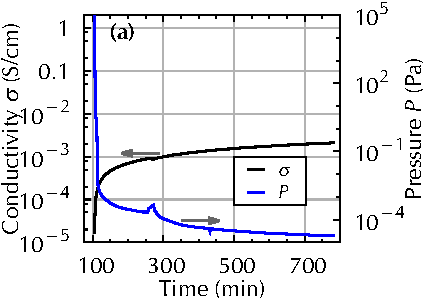
\includegraphics{plot/killing+reanimating-C60-2-evap}%
\hfill
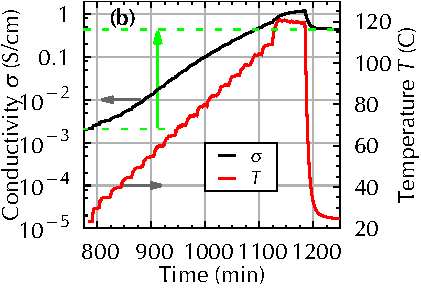
\includegraphics{plot/killing+reanimating-C60-3-heat}%
\setcapwidth[c]{\tmCapWidth}%
\caption
[Conductivity regeneration by vacuum and \insitu heat treatment]
{Conductivity regeneration by (a) vacuum and (b) \insitu heat treatment.}
\label{fig:killing+reanimating-C60-2+2}
\end{figure}
%
After this measurement, the sample is stored again in the vacuum chamber and the pumps are connected and switched on again, evacuating the chamber for several hours. Monitoring the conductivity, an increase up to a value of \c[2.1E-3] is observed at a pressure of \pa{2E-5}, shown in \figref{killing+reanimating-C60-2+2}\,(a).
Hence, 0.1\% of the initial conductivity is restored by the vacuum, indicating that the molecular n-doping is still partly intact.

An additional, much stronger restoring of the conductivity is achieved by slowly heating the sample in vacuum up to \grad{120}, in steps of \K{5} and 20~minutes at each temperature. As shown in \figref{killing+reanimating-C60-2+2}\,(b), W
the conductivity rises significantly with temperature. Cooling the sample back down to \grad{25}, the conductivity stayed at a level of \c[0.44]. Applying several longer cycles of heating to \grad{120} and cooling down to \grad{25} a saturation at \c[0.60] is found.

In conclusion, the initial conductivity of \c[1.88] (\mbox{$100\,\%$}) decreased to \c[1.7E-5] (\mbox{$\approx0.001\,\%$}) after 16~minutes in air. By vacuum treatment \c[2.1E-3] (\mbox{$\approx0.1\,\%$}) and by heat treatment \c[0.60] (\mbox{$\approx32\,\%$}) are restored.

The annealing and removal of oxygen- and hydrogen-related electron traps in pure \CS has already been investigated by the thermally stimulated current (TSC) technique and validated by an enhanced OFET-mobility of four orders of magnitude when thermally annealed after air-exposure\cite{Matsushima2007}. Since for the above discussed sample more than 30\,\% of the initial conductivity is restored by vacuum and heat treatment, it is concluded that the n-doping stays at least partly intact during the air-exposure and is only compensated by oxygen-related traps and p-doping effects.

The same sample is later exposed to air for 3~hours to check for the longtime effects. Again, a drop in conductivity is measured, down to a value of \c[6.6E-7]. Re-evacuating the vacuum chamber leads to \c[2.3E-5] and heat treatment to \c[0.03]. Thus, the much longer air-exposure reduces the final conductivity by an additional factor of 20. The final value is still above the conductivity of a freshly fabricated and thermally annealed sample of \CS doped by \C[0.014] of the air-stable precursor n-dopant \aob that will be presented and discussed in the following chapter. However, it seems evident that the longer exposure degrades more \WPd molecules within the \CS layer.

%
\begin{table}[b]
\centering
\caption
[Effect on air-exposure on \c, \Es and \Eact]
{Overview of the effect on air-exposure on the observables conductivity \c, Seebeck coefficient \S, \EsLong \Es and \EactLong \Eact. All measurements performed on the same sample of \C[0.033] \WPd.}
\label{tab:Pd-Killing}
\begin{tabular}{
c%
c%S[tabnumalign=centre,tabformat=1.2]%
c%S[tabnumalign=centre,tabformat=3.1]%
c%S[tabnumalign=centre,tabformat=3.1]%
c%S[tabnumalign=centre,tabformat=3.1]%
}
\toprule
 & {\c} & {\S} & {|\Es|} & {\Eact}%
\\
measurement after & { \si{\siemens\per\centi\meter}}
 & { \si{\micro\volt\per\kelvin}}
 & { \si{\milli\electronvolt}}
 & { \si{\milli\electronvolt}}
% & { \uVK{}} & { \meV{}} & { \meV{}}
 \\
\midrule %hspace{0.9ex}
 & {($\T[25]$)} & \multicolumn{2}{c}{(\Tm[40])}    & {($\T=25 \text{ to } \grad{70}$)}\\
%
sample preparation
& 2.27
 & & & \\
annealing at \grad{70}
& 2.90
 & $-226.1$
 & \hspace*{1ex}67.7
 & \hspace*{1ex}77.8 \\ 
several loops \grad{25} to \grad{100}
& 1.78
 & $-234.8$
 & \hspace*{1ex}73.5
 & \hspace*{1ex}99.6 \\ 
60\,min at \grad{120}
& 1.88
 &  &     &   \\
16\,min in air
 & \num{1.7E-5}
 &
 &
 &\\
th. annealed in vacuum
 & 0.60 
 & $-262.8$
 & \hspace*{1ex}82.3
 & 103.4 \\ 
180\,min in air
 & \num{6.6E-7}
 &
 &
 & \\
th. annealed in vacuum
 & 0.03
 & $-352.2$
 & 110.3
 & 146.5 \\ 
%
\bottomrule
\end{tabular}
\end{table}
%
%
Besides the conductivity, the \EsLongL and the \EactLongL are measured after vacuum and heat treatment. A summary is given in \tabref{Pd-Killing}. The initial conductivity dropped by a factor of 3 after 16~minutes in air and by an additional factor of 20 after 3~hours in air. 16~minutes in air increased $|\Es|$ by \meV{8.8} to \meV{82.3} ($+12\,\%$) and \Eact by \meV{3.8} to \meV{103.4} ($+4\,\%$). The second exposure of 3~hours in air leads to a gain of $|\Es|$ by another \meV{28.0} ($+34\,\%$) and of \Eact by \meV{43.1} ($+42\,\%$).

The rise in $|\Es|$ corresponds to an increased difference between the \EfLongL and the \EtLongL and hence to a smaller \neLongL. However, after 3~hours of air-exposure the observed $|\Es|$ of the investigated sample of \C[0.033] of \WPd is still lower than the corresponding value of an unexposed sample with a tenth of the \CLong: \mbox{$|\Es|=\meV{167}$} at \C[0.004]. This comparison clearly shows that for the air-exposed sample, at least 10\,\% of the \WPd molecules survive the contact with air and are still providing molecular n-doping. As the measured Seebeck coefficients \S are still negative, compensating p-doping of \CS by oxygen can be excluded.
While the \Es is already strongly affected by 16~minutes of air-exposure, the \Eact only significantly increases after the 3~hours exposure. This suggests a slow but strong change of the charge carrier mobility due to a sustainable formation of electron traps, whereas in case of short exposure most of the induced electron traps can be removed by thermal annealing in vacuum. Furthermore, the larger amount of degradation products that are expected to be present in the layer after 3~hours of air-exposure could act as additional trap states and hence raise \Eact.

Further studies of the degradation mechanism of pure \WPd as well as of layers of \CS doped by \WPd employing the techniques of ultraviolet photoelectron spectroscopy (UPS), X-ray photoelectron spectroscopy (XPS) as well as laser desorption/ionization time of flight mass spectrometry (LDI-TOF-MS) revealed that the majority of the dopant molecules immediately decomposes after air-exposure\cite{TietzeMenke2013}.
However, the remaining \WPd molecules stay intact and slowly degrade with an exponential decay time of \mbox{$\approx13$~minutes}. These findings are attributed to a rise of the IE of \WPd upon charge-transfer, resulting in a protection against oxidation in air.
Consequently, the observed recovery of the conductivity is interpreted as a self-passivation of the molecular n-doping.
Such a passivation mechanism of n-doped layers enables processing steps under ambient conditions, greatly enhancing device fabrication possibilities\cite{Kleemann2012}.

% \pagebreak
\section{Conclusion}\label{sec:ResPdConclusion}
It is found that both dopants, \CrPd and \WPd, are well suited to n-doped \CS. Extremely high conductivities of up to \c[7] are measured, with \CrPd leading to larger values than \WPd. Continuously probing the conductivity for 1~hour after sample preparation, an increase for low and a decrease for high \CLongs is observed. In order to ensure comparable measurement conditions, the samples are thermally annealed prior to the electrical investigations. Afterwards, for both dopants a linear relation of $\c(\C)$ is measured, until at high \C a drop in \c is detected. This reduction is attributed either to a disturbance of the morphology by the large amount of dopants in the layer and hence a drop of the mobility or to a reduced doping efficiency due to clustering of dopants. Seebeck data showed that \S decreases further at high \C and hence the \neLong increases, which suggests that the doping efficiency is not decreasing and the drop in conductivity is due to a reduced mobility. 

Such high conductivities are relevant for device applications, since they enable good charge injection and extraction from the contacts, hence reducing ohmic losses and increasing device performance\cite{Blochwitz1998}.
Furthermore, the substitution of the metal contacts by highly conducting doped organic layers would allow for pure organic devices\cite{Schubert2013}. Additionally, in organic tandem photovoltaic cells, a highly conducting recombination and spacer layer between the two subcells is crucial for device performance\cite{Riede2011,Meiss2011}.

Varying the temperature, the conductivity is found to be in good agreement with a thermally activated hopping transport and an \EactLong \Eact is derived. \Eact decreases with \C for low and moderate \C of both dopants, attributed to a shift of the \EfLong towards the \EtLong. At high \C, the \Eact increases, indicating a disturbance of the morphology of the host material by the large percentage of dopant molecules, in agreement with the conductivity data.

Thermoelectric measurements prove that for all samples electrons are the dominating charge carriers and allow for deriving the energetic difference \Es between \EfLong and \EtLong. This difference is reduced with raising \CLong, as expected from the trend of \Eact. As \Es does not increase at high \C, the observed rise of \Eact and the reduced \c are attributed to changes in the mobility.

AFM studies of the surface roughness yield a rising surface roughness with \CLong in the low and medium doping regime. At high \C, the surfaces are found to be very smooth, which is attributed to a hydrogen film on the surface, attracted by the strongly ionizing dopants and shielding the real topography. Hence, AFM is not a suitable technique to study the morphology of doped layers, as only the surface is probed and material content cannot be resolved.

Air-exposure of n-doped layers is found to lead to fast degradation of the \cLong. However, a large fraction of the initial conductivity can be restored by vacuum and heat treatment. This finding could allow for device processing steps under ambient conditions, greatly enhancing device fabrication possibilities.

Overall it is shown that both dopants are exceptionally well suited for n-doping \CS. Recently, \WPd was successfully deployed in devices \cite{Schunemann2012,Fischer2012}. It would be interesting to study these dopants in hosts of lower \EA to investigate the influence of the molecules' energy levels. First measurements of successfully n-doping ZnPc\footnote{ZnPc is zinc phthalocyanine, $\text{EA}=\eV{3.34}$\cite{Gao2001}} by \WPd\cite{Burtone2013} are promising.

